% !Mode:: "TeX:UTF-8"
% !TEX program = xelatex
\documentclass[a4paper]{article}
\usepackage{amsmath}
\usepackage{amssymb}
\usepackage{ctex}
%\usepackage{braket}
%\usepackage[european]{circuitikz}
\usepackage{multirow}
\usepackage{float}
\usepackage{graphicx}
\usepackage{sidecap}
\usepackage[justification=centering]{caption}
\usepackage{geometry}
\geometry{left=2.5cm,right=2.5cm,bottom=2.5cm,top=2.5cm}
\title{近代物理实验报告8.4:蒸汽冷凝法制备纳米颗粒}
\author{林杨\quad 211840092\quad 物理学院}
\date{2024年3月23日}
\begin{document}
\maketitle
\bibliographystyle{unsrt}
%--------main-body------------

\section{引言}
在物理学发展的历史上,人类对宏观领域和微观领域已经进行了长期的、不断深入的研究。然而介于宏观和微观之间的所谓介观领域却是一块长期以来未引起人们足够蜇视的领域。这一领域的特征是以相干量子输运现象为主,包括团簇、纳米体系和亚微米体系,尺寸范围约为1$\sim$1000nm。
但习惯上人们将100$\sim$1000nm范围内有关现象的研究。特别是电输运现象的研究领域称为介观领域。因而l$\sim$100nm的范围就特指为纳米尺度,在此尺度范围的研究领域称为纳米体系(图(\ref{fig1}))。
\begin{figure}[!ht]
\centering
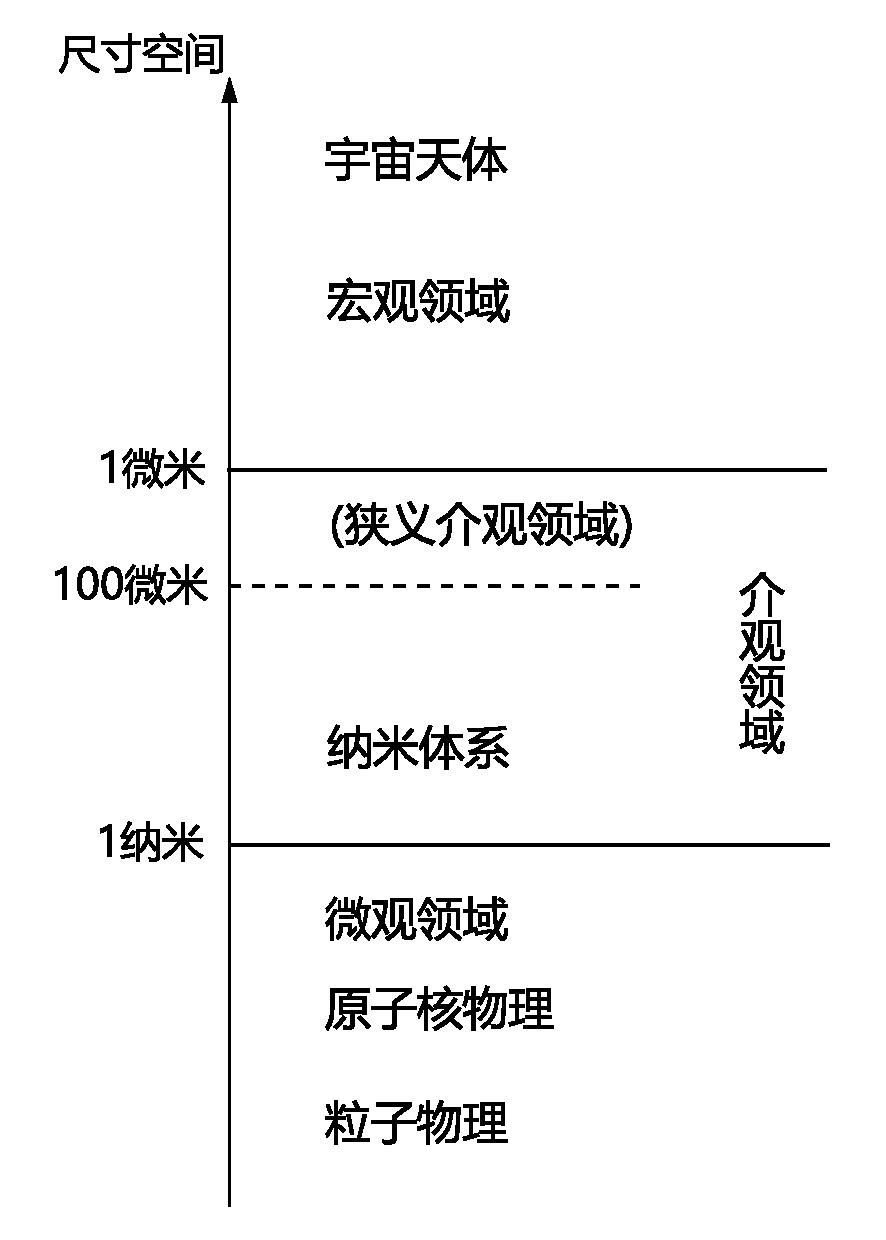
\includegraphics[width=0.4\textwidth]{fig/fig1.pdf}\\
\caption{纳米体系的尺寸空间}\label{fig1}
\end{figure}

纳米科技正是指在纳米尺度上研究物质的特性和相互作用以及利用这些特性的科学技术。经过近十几年的急速发展。纳米科技已经形成纳米物理学、纳米化学、纳米生物学、纳米电子学、纳米材料学、纳米力学和纳米加工学等学科领域。纳米材料与宏观材料相比具有以下的一些特殊效应。
\subsection{小尺寸效应}
纳米材料的尺度与光波波长、德布罗意波长以及超导态的相干长度或透射深度等物理特征尺寸相当或更小,宏观晶体的周期性边界条件不再成立,导致材料的声、光、电、磁、热、力学等特性呈现小尺寸效应。例如各种金属纳米颗粒几乎都显现黑色。表明光吸收显著增加;许多材料存在磁有序向无序转变,导致磁学性质异常的现象;声子谱发生改变,导致热学、电学性质显著变化。曾有人利用高分辨率电子显微镜追踪拍摄超细金微粒,观察到微粒的外形、结晶态不停地变化。特定界面的原子不断地脱离平衡位置又不停地返回平衡位置,呈现出与常规材料不同的特性,被称为living particle。纳米微粒之间甚至在室温下就可以合二为一,它们的熔点降低自然是意料中的结果。图(\ref{fig2})为金微粒熔点与尺寸的关系。
\begin{figure}[!ht]
\centering
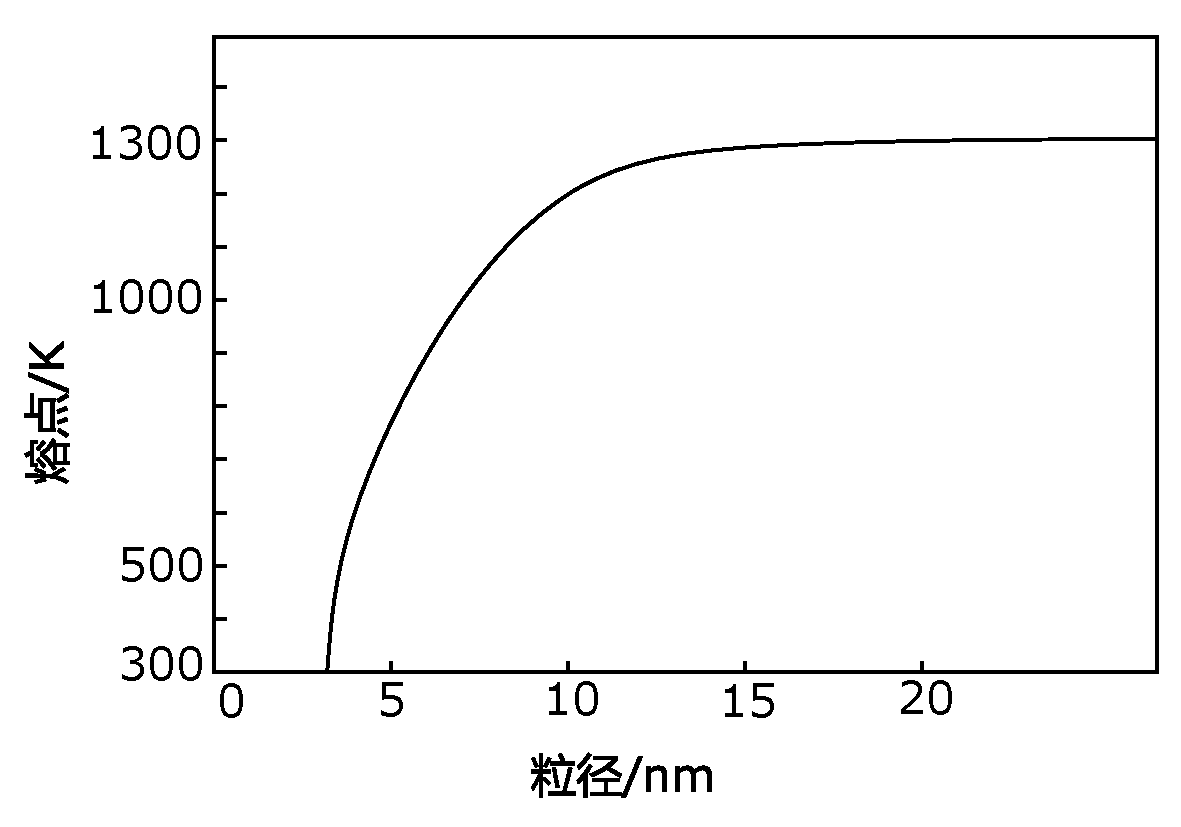
\includegraphics[width=0.7\textwidth]{fig/fig2.pdf}\\
\caption{金微粒熔点与粒径的关系}\label{fig2}
\end{figure}

\subsection{表面效应}
以球形颗粒为例。单位质量材料的表面积(称为比表面积)反比于该颗粒的半径。因此当半径减小时比表面积增大。例如将一颗直径1$\mu$m的颗粒分散成直径10nm的颗粒,颗粒数变为100万颗,总比表面积增大100倍。表面原子数比例、表面能等也相应地增大。从而表面的活性增高。洁净的金属纳米微粒往往会在室温环境的空气中燃烧(表面有薄层氧化物时相对稳定),这是必须面对的问题。但是反过来也为优良的催化剂提供了现实可能。
\subsection{量子尺寸效应}
传统的电子能带理论表明,金属费米能级附近电子能级是连续的。但是按照著名的久保(kubo)理论。低温下纳米微粒的能级不连续。相邻电子能级间距$\delta$与微粒直径相关
\begin{equation}
\delta = \frac{4}{3}\frac{E_F}{N}\label{eq1}
\end{equation}
式中N为一个微粒所包含的导电电子数。$E_F$为费米能
\begin{equation}
E_F = \frac{\hbar}{2m}\left(3\pi^2n\right)^{\frac{2}{3}}\label{eq2}
\end{equation}
式中$\hbar$为普朗克常数。m为电子质量。N为电子密度。若将微粒简单地看作球形的,则近似地
\begin{eqnarray}
\delta \propto \frac{1}{d^3}\label{eq3}
\end{eqnarray}
d为直径。由此可见随着微粒直径变小,电子能级间距变大。久保理论中提及的低温效应按如下标准判断,即只在$\delta > k_BT$时才会产生能级分裂。式中$k_B$为玻尔兹曼常数,T为绝对温度。这种当大块材料变为纳米微粒时,金属费米能级附近的电子能级由准连续变为离散能级的现象称为量子尺寸效应。当能级间距大于热能、磁能、静磁能、静电能、光子能槛或超导态的凝聚能时。微粒的磁、电、光、声、热以及超导电性均会与大块材料有显著不同。以Cu纳米微粒为例,其导电性能即使在室温下也明显下降。对于半导体微粒,如果存在不连续的最高被占据分子轨道和最低未被占据的分子轨道能级,能隙变宽现象等亦称为量子尺寸效应。
\subsection{宏观量子隧道效应}
微观粒子具有穿透势垒的几率,称为隧道效应。近年来,人们发现一些宏观量,例如小颗粒的磁化强度,量子相干器件中的磁通量等亦具有隧道效应,称为宏观量子隧道效应。宏观量子隧道效应对纳米科技有看重要的价值,它是纳米电子学发展的重要基础依据。
此外,近十多年来,尚有“库仑堵塞与量子隧穿”、“介电限域效应”等新效应被发现。上述各种效应使得纳米材料呈现出与宏观材料显著不同的特性,甚至出现一些反常的现象,更加吸引着人们开拓和探索这一引人入胜的学科领域。
在整个纳米科技的发展过程中,纳米微粒的制备和微粒性质的研究是最早开展的。时至今日,纳米科技的领域已经迅速地扩大和深入,但要进入纳米领域,最好还是从纳米微粒的制备与测量起步。

\section{实验目的}
\begin{enumerate}
\item 学习和掌握利用蒸汽冷凝法制备金属纳米微粒的基本原理和实验方法,研究微粒尺寸与惰性气体气压之间的关系。
\item 学习利用电子成像法、X射线衍射峰宽法或其它方法测量微粒的粒径。
\end{enumerate}

\section{实验仪器}
HT-218型纳米微粒制备实验仪。

\section{实验原理}
利用宏观材料制备微粒,通常有两条路径。一种是由大变小,即所谓粉碎法;一种是由小变大,即由原子气通过冷凝、成核、生长过程,形成原子簇进而长大为微粒,称为聚集法。由千各种化学反应过程的介入,实际上已发展了多种制备方法。
\subsection{粉碎法}
图(\ref{fig3})示意几种最常见的粉碎法。
\begin{figure}[!ht]
\centering
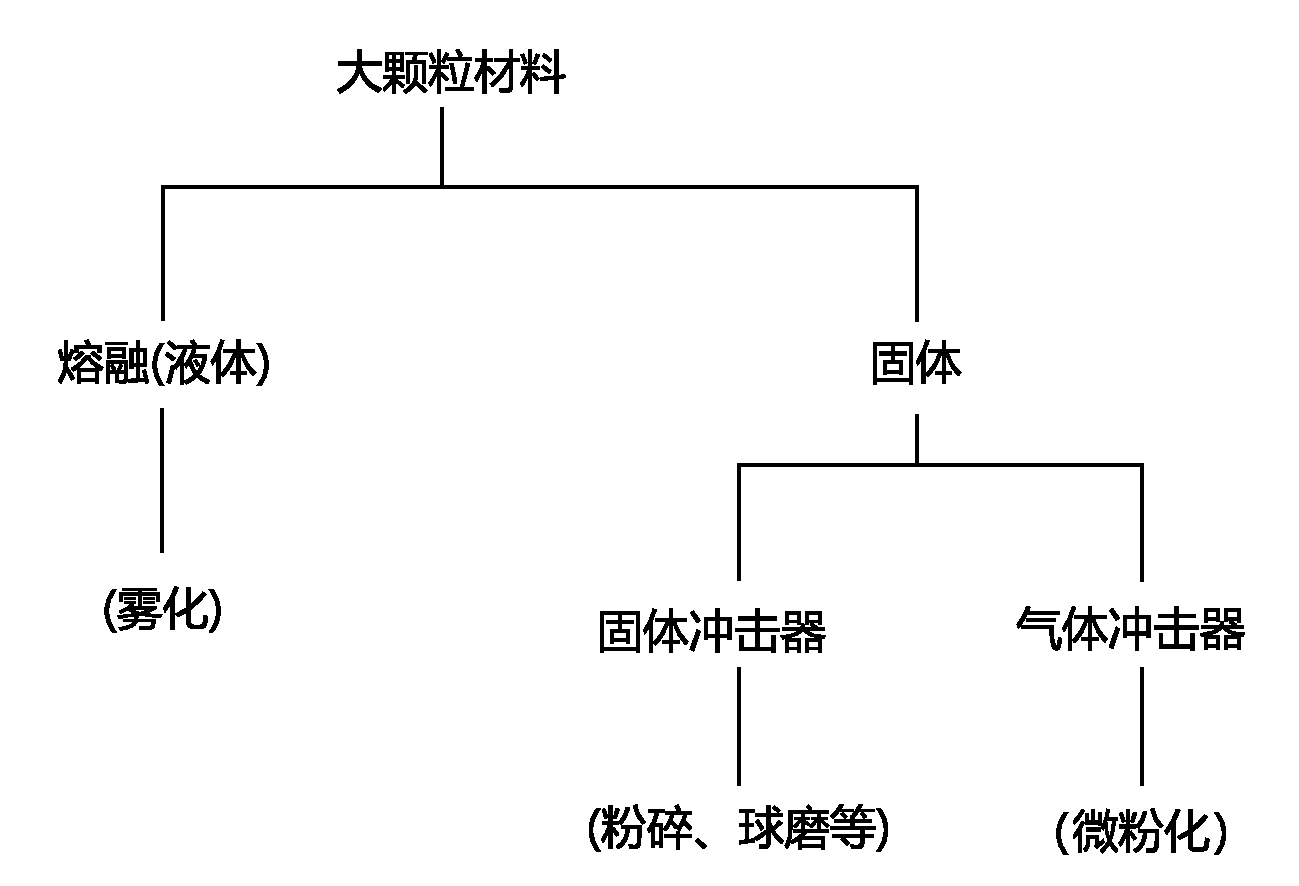
\includegraphics[width=0.6\textwidth]{fig/fig3.pdf}\\
\caption{粉碎法}\label{fig3}
\end{figure}

实验室使用得最多的是球磨粉碎。球磨粉碎一开始粒径下降很快,但粉碎到一定程度时,由冷焊或冷烧结引起的颗粒重新聚集过程与粉碎过程之间达到动态平衡,粒径不再变小。进一步细化的关键是阻止微晶的冷焊。这往往通过添加助剂完成。1988年,Shingu等利用高能球磨法成功地制备了Al-Fe纳米品。发展至今。对于bcc结构的材料(如Cr、Fe、W等)和hcp结构的材料(如Zr、Ru等)的纳米微粒较易制备,但具有fcc的材料(如Cu)难以形成纳米微晶。球磨粉碎法的缺点是微粒尺寸的均匀性不够,同时可能会引入杂质成分。但相对而言工艺较简单,产率较高。而且还能制备一些其它方法无法制备的合金材料。
\subsection{化学液相法}
化学液相法制备纳米微粒获得很大的进展,目前已发展成共沉淀法、水热法、冻结干燥法、溶胶一凝胶法等。利用化学液相法已制备成许多种类的纳米金属、非金属单品微粒及各种氧化物、非氧化物以及合金(如CoFeO$_4$,BaTiO$_3$)、固溶体(如Al$_2$O$_3$-TiO$_2$)。
\subsection{气相法(聚集法)}
气相法制备纳米微晶可以追溯到古代。我们的祖先就曾利用蜡烛火焰收集炭黑制墨。文献记录表明,1930年代,Rufud为了研究红外吸收,在空气中制备了Ni等11种金属的纳米微粒。1962年,由于日本物理学家Kubo(久保)提出量子尺寸效应,引起了物理学工作者的极大兴趣,促进了纳米微粒的制备及检测。1963年kimoto等在稀薄氢气氛的保护下利用金属加热蒸发再冷凝,成功地制备了20多种金属材料的纳米微粒。时至今日,除了在加热方法上已发展了电阻加热法、等离子喷射法、溅射法、电弧法、激光法、高频感应法及爆炸法等各种方法,在制备原理上亦已发展了CVD法、热解法及活性氢—熔融金属反应法等。它们为不同的用途,提供各自适宜的制备方法。
\begin{SCfigure}[][ht]
\centering
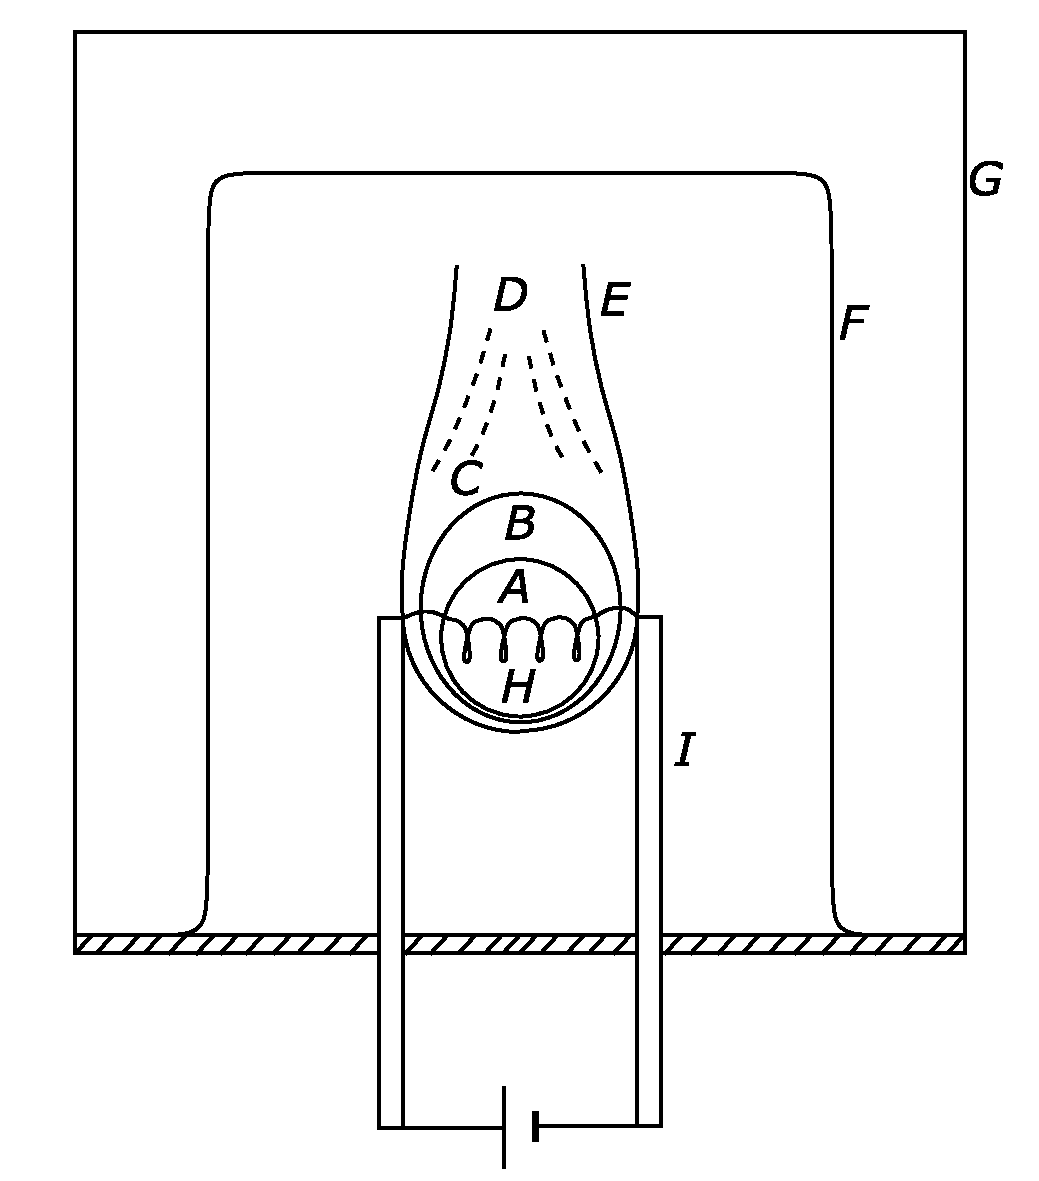
\includegraphics[width=0.5\textwidth]{fig/fig4.pdf}
\caption{蒸气冷凝法原理\\A. 原材料的蒸汽;B. 初始成核;C. 形成纳米微晶;D. 长大了的纳米微粒;E. 惰性气体,气压约为kPa量级;F. 纳米微粒收集器;G. 真空罩;H. 加热钨丝;I. 电极}\label{fig4}
\end{SCfigure}

在各类制备方法中。最早被采用并进行较细致实验研究的是蒸汽冷凝法。图(\ref{fig4})显示蒸气冷凝法制备纳米微粒的过程。首先利用抽气泵对系统进行真空抽吸,并利用惰性气体进行置换。惰性气体为高纯Ar、He等,有些情形也可以考虑用N$_2$气。经过几次置换后,将真空反应室内保护气的气压调节控制至所需的参数范围,通常约为0.lkPa至10kPa范围,与所需粒子粒径有关。当原材料被加热至蒸发温度时(此温度与惰性气体压力有关,可以从材料的蒸汽压温度相图查得)蒸发成气相。气相的原材料原子与惰性气体的原子(或分子)碰撞。迅速降低能蜇而骤然冷却。骤冷使得原材料的蒸汽中形成很商的局域过饱和,非常有利于成核。图(\ref{fig5})显示成核速率随过饱和度的变化。成核与生长过程都是在极短的时间内发生的,图(\ref{fig6})给出总自由能随核生长的变化。一开始自由能随着核生长的半径增大而变大,但是一x旦核的尺寸超过临界半径,它将迅速长大。

首先形成原子簇,然后继续生长成纳米微晶,最终在收集器上收集到纳米粒子。为理解均匀成核过程,可以设想另一种情形,即抽掉惰性气体使系统处于高真空状态。如果此时对原材料加热蒸发,则材料蒸汽在真空中迅速扩散并与器壁碰撞而冷却,此过程即是典型的非均匀成核,它主要由容器壁的作用促进成核、生长并淀积成膜。而在制备纳米微粒的过程由于成核与生长过程几乎是同时进行的,依粒的大小与饱和度P/Pe有密切关系,这导致如下几项因素与微粒尺寸有关。(1)惰性气体的压力。压力越小碰撞几率越低。原材料原子的能益损失越小。Pe值降低较慢。(2)惰性气体的原子昼越小,一次碰撞的能量损失越小。(3)蒸发速率越快,P/Pe越大。(4)收集器离蒸发源越远,微粒生长时间越长。实际操作时可根据上述几方面的因素调剂P/Pe值,从而控制微粒的分布尺寸。
\begin{figure}[!ht]
\begin{minipage}{0.48\textwidth}
\begin{center}
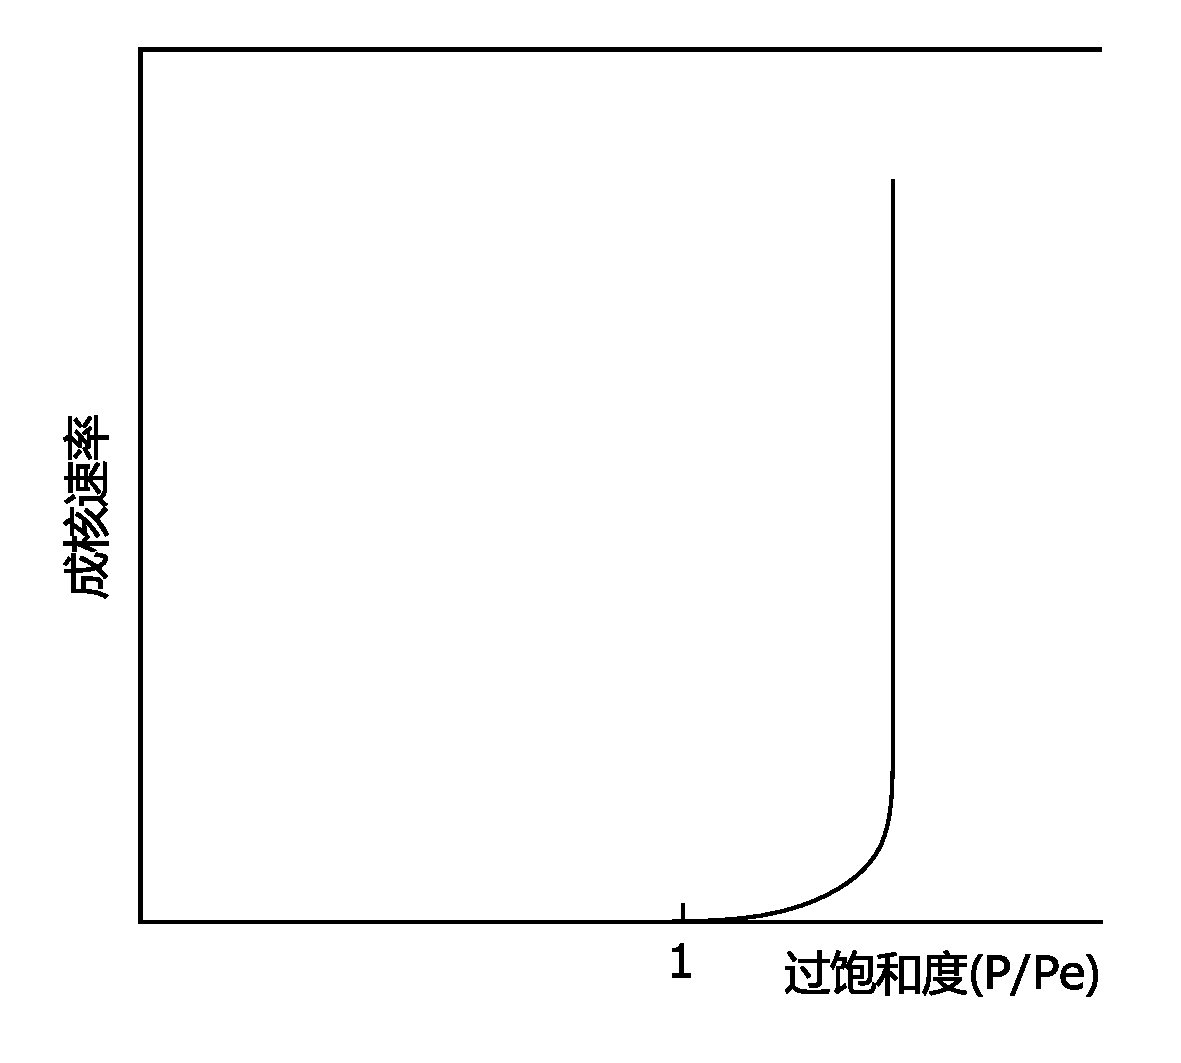
\includegraphics[width=0.95\textwidth]{fig/fig5.pdf}\\
\caption{成核速率随过饱和度的变化}\label{fig5}
\end{center}
\end{minipage}
\begin{minipage}{0.48\textwidth}
\begin{center}
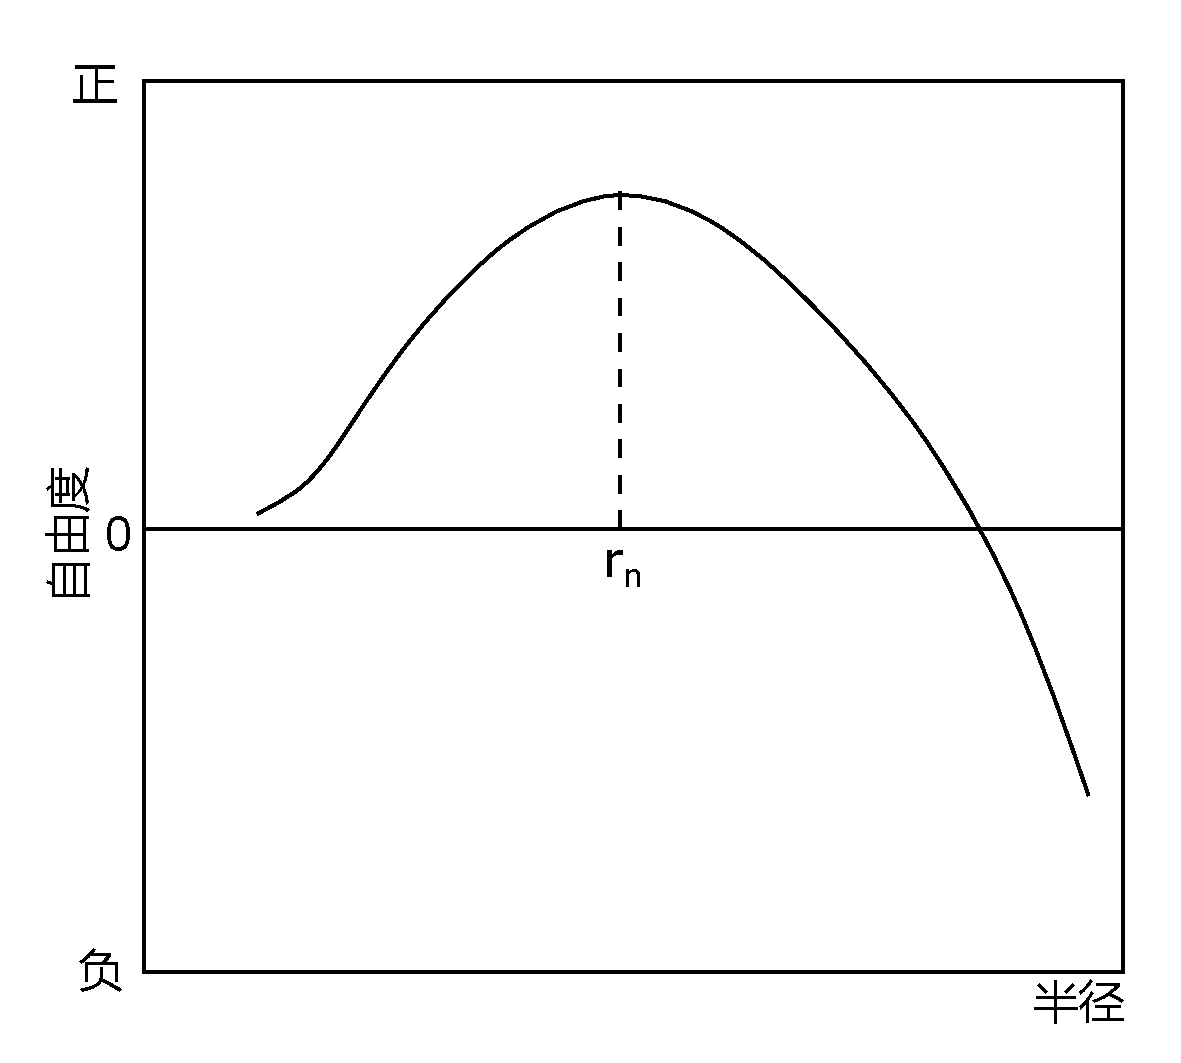
\includegraphics[width=0.95\textwidth]{fig/fig6.pdf}\\
\caption{总自由能随核生长的变化}\label{fig6}
\end{center}
\end{minipage}
\end{figure}

\section{实验内容}
\subsection{准备工作}
\begin{enumerate}
\item 检查仪器系统的电源接线、惰性气体连结管道是否正常。惰性气体最好用高纯Ar气,亦可考虑使用化学性质不活泼的高纯N$_2$气。
\item 利用脱脂白绸布、分析纯酒精、仔细擦净真空罩以及罩内的底盘、电极和烧杯。
\item 将螺旋状钨丝接至铜电极。
\item 从样品盒中取出铜片(用于纳米铜粉制备),在钨丝的每一圈上挂一片,罩上烧杯。
\item 罩上真空罩,关闭阀门$V_1$,$V_2$,将加热功率旋钮沿逆时针方向旋至最小,合上电源总开关$S_1$。此时真空度显示器显示出与大气压相当的数值,而加热功率显示值为零。
\item 合上开关$S_2$,此时抽气单元开始工作,电磁闭$V_e$自动接通,真空室内压力下降。下降至一定值时关闭$S_2$,观察真空度是否基本稳定在该值附近,如果真空度持续变差,表明存在漏气因素,检查$V_1$,$V_2$是否关闭。正常情况下不应漏气。
\item 打开阀门$V_1$。此时惰性气进入真空室,气压随之变大。
\item 熟练上述抽气与供气的操作过程,直至可以按实验的要求调节气体压力。
\item 准备好备用的干净毛刷和收集纳米微粉的容器。
\end{enumerate}
\subsection{制备铜纳米微粒}
\begin{enumerate}
\item 关闭$V_1$、$V_2$阀门,对真空室抽气至0.05kpa附近。
\item 利用氢气(或氮气)冲洗真空室。打开阀门$V_1$,使氩气(或氮气)进入真空室,边抽气边进气(氩气或氮气)约5分钟。
\item 调节阀$V_1$,观察真空度基本稳定在0.13kpa附近。
\item 沿顺时针方向缓慢旋转加热功率旋钮,观察加热功率显示器,同时关注钨丝。随着加热功率的逐渐增大。钨丝逐渐发红进而变亮。当温度达到铜片(或其它材料)的熔点时铜片熔化,并由于表面张力的原因,浸润至钨丝上。
\item 继续加大加热功率时可以见到用作收集器的烧杯表面变黑,表明蒸发已经开始。随着蒸发过程的进展,钨丝表面的铜液越来越少,最终全部蒸发掉,此时应立即将加热功率调至最小。
\item 打开阀门$V_2$使空气进入真空室,当压力与大气压最近时,小心移开真空罩,取下作为收集罩的烧杯。用刷子轻轻地将一层黑色粉末刷至烧杯底部再倒入备好的容器,贴上标签。收集到的细粉即是纳米铜粉。
\item 在2$\times$0.13kpa及3$\times$0.13kpa处重复上述实验步骤制备,记录每次蒸发时的加热功率,观察每次制备时蒸发悄况有何差异。
\end{enumerate}

\section{注意事项}
\begin{enumerate}
\item 实验中加热时间不可过长,否则铜可能颗粒过大产生金属光泽。
\item 使用阀门$V_1$、$V_2$时力量应适中,不要用暴力猛拧,但也不要过分谨慎不敢用力以至阀门不能完全关闭。通过实验的实际操作过程,提高基本的实验能力。
\item 蒸发材料时,钨丝将发出强烈耀眼的光。其中的紫外部分已基本被玻璃吸收。在较短的蒸发时间内用肉眼观察未见对眼睛的不良影响。但为安全起见。请尽量带上保护限镜。
\item 制成的纳米微粉极易弥散到空气中。收集时要尽量保持动作的轻慢。
\item 若需制备其它金属材料的纳米微粒,可参照铜微粒的制备。但熔点太高的金属难以蒸发,而铁、锦与钨丝在翡温下易发生合金化反应,只宜闪蒸,即快速完成蒸发。
\item 亦可利用低气压空气中的氧或低气压氧,使钨丝表面在称温下局部氧化并升华制得氧化钨微晶。
\item 因真空泵为油泵,不能直接对大气抽气(所有阀门关上)以免喷油。加热后的钨丝很脆,容易折断,务必小心!如要清洁在真空中加热即可。
\end{enumerate}

\section{实验中出现的现象和实验结果}
\begin{enumerate}
\item 加热开始后,挂在钨丝上的铜条熔断成两段并掉落。铜条与钨丝接触的部分,大部分升华为铜蒸汽,少部分熔化为液体。关闭加热后,这部分液体会凝固成铜小球,挂在钨丝上。
\item 加热开始后,容器内气压会有所升高;加热结束后,气压将下降至原气压以下。
\item 加热开始后,容器内会产生“黑烟”。随着容器内真空条件的下降,这一现象会愈加明显。
\item 加热结束时,容器内的铜蒸汽立刻凝华,烧杯壁呈现黑色。将这一层黑色颗粒刮在面纸上。由图(\ref{fig7})可以发现,颗粒颜色有些许差异,但未发现和实验的真空条件有直接关联。
\item 其他实验结果见图(\ref{fig7})。图片被划分为两行三列。按列来看,从左到右,对应气压逐渐增大的三组实验。按行来看,每一列的上方为纳米颗粒附着在烧杯上的照片,下方为用毛刷将颗粒刮下后的照片。
\end{enumerate}

\begin{figure}[!ht]
\centering
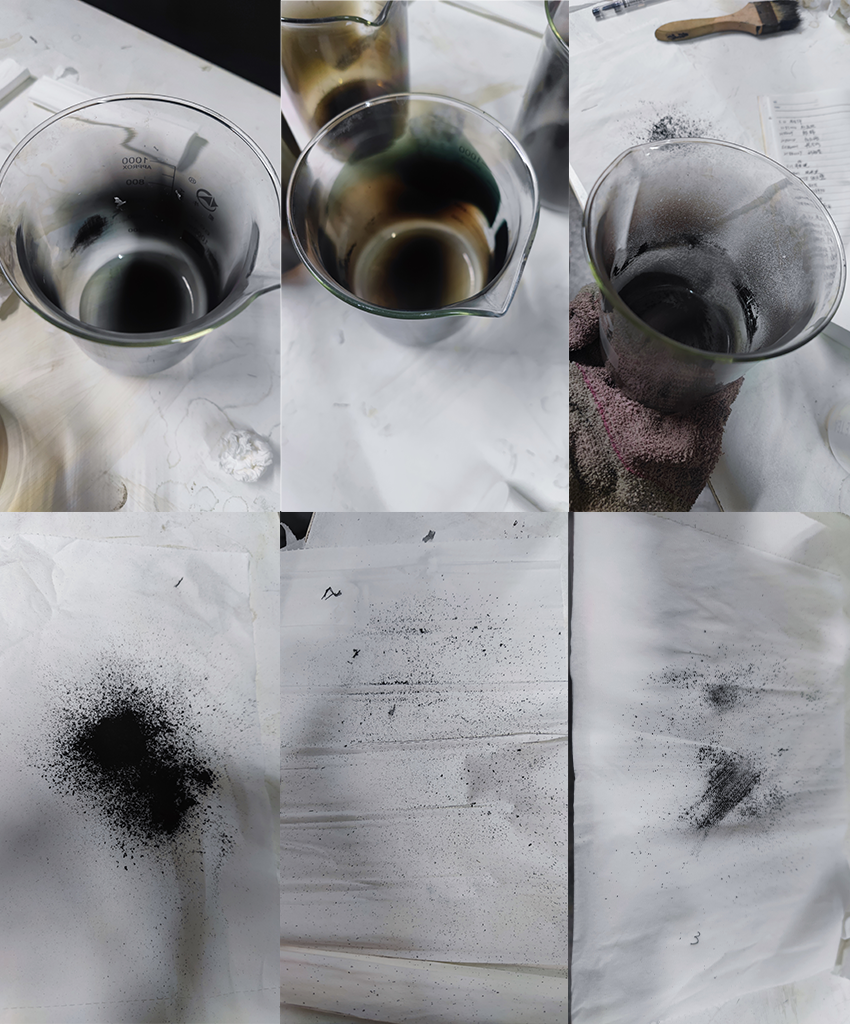
\includegraphics[width=0.7\textwidth]{img/final.png}\\
\caption{三组实验分别得到的烧杯和纳米颗粒}\label{fig7}
\end{figure}


\section{思考题}
\subsection{真空系统为什么应保持清洁?}
\begin{enumerate}
\item 系统内残留的少量气体应保持清洁,这保证了铜蒸汽只在烧杯壁上凝华。如果系统内残留有不纯的气体,铜蒸汽可能会在非均匀的条件下直接凝华在气体凝结核上。
\item 烧杯壁应保持清洁,这防止了脏污或烧杯内残留颗粒的干扰。光滑清洁的烧杯壁也保证了铜蒸汽凝华的均匀性。
\end{enumerate}


\subsection{为什么对真空系统的密封性有严格要求?如果漏气,会对实验有什么影响?}
如果漏气,铜在升华和凝华时的压强条件就会发生改变,实验就会失败。如果漏入活泼气体,则会产生更严重的安全隐患。
\subsection{为什么使用氮气纯度要求很高?}
如果惰性气体中掺杂有氧气等活泼气体,铜便会在高温下氧化,实验就会失败。
\subsection{为什么要利用纯净氮气对系统进行置换、清洗?}
一个压强由惰性气体产生的系统比一个压强由活泼气体产生的系统更加安全。
\subsection{从成核和生长的机理出发,分析不同保护气气压对微粒尺寸有何影响?}
在稀薄气体模型中,气压正比与气体粒子的数密度。因此,气压越大,铜蒸汽原子越容易与气体分子碰撞形成大尺寸颗粒。形成的大尺寸颗粒更容易与新的铜蒸汽原子碰撞,最终形成大型铜微粒。因此,气压越高,最终生成的铜颗粒尺寸会更大。
\subsection{为什么实验制得的铜微粒呈现黑色?}
纳米颗粒不再具有晶体的宏观性质。纳米颗粒对光的吸收会更大,反射更少。最终呈现出黑色。
\subsection{实验制得的铜微粒的尺寸与气压之间成何关系?为什么?}
见8.5题。
\subsection{实验中在不同气压下蒸发时,加热功率与气压之间成何关系?为什么?}
理论上,压力越高,铜的蒸发点越高,需要的加热功率越高。实际上,器材的加热功率远远超过了所需的功率,故无需太过在意这一点。
\subsection{在不同气压下蒸发时。观察到微粒“黑烟”的形成过程有何不同?为什么?}
气压越高,“黑烟”现象越明显。原理同8.5题。

\nocite{jiaocai}
\bibliography{ref}
\end{document}